\documentclass[12pt]{report}
\usepackage[utf8]{inputenc}
\usepackage{graphicx}

\title{A Comprehensive Guide to Start Building an IoT Product}

\begin{document}
%% chapter normaly 
\chapter{What are smart network?}

Let’s take a simple example. Your phone. Before it was connected to the Internet it was dumb, like really dumb. It could only play the songs you have put in it. It could only call the people you have the contact number for.

\textit{Then something magical happened. We connected it to the internet}

Now it can play any song. You are not limited to just a contact number for connecting to someone. You have access to information in your hand that won’t fit in TBs of data storage. That’s the power of connecting to the Internet.

Internet and smartphones, computers are really powerful tools, but the smartphone won’t water your plants, it won’t open your door. These devices have very limited physical abilities.

The Internet of Things is about extending the power of the internet beyond computers and smartphones to a whole range of other things, processes, and environments.

\section{How do we do that? How do we extend the power to the internet?}
By putting components in the world around you which interact and sense the physical world and connecting those to the internet. These components are combinations of sensors and actuators.

\section{What is the sensor?}
Simply put, the sensor measures a physical property. Like temperature sensor measures temperature.

\section{What is an actuator?}
You can understand actuators as the opposite of the sensor. Like sensors converts external changes to signal, actuators convert signature to action. Like opening a door lock.

Of course with these sensors and actuators you would need some additional hardware that controls these and if needed and transfers information.

%%chapter normaly
\section{IoT Changing the world}
IoT enables you to monitor and act on connected devices more closely than ever. Be it industries managing their machines, farmers checking on their crops, governments managing the borders, administrations monitoring air or water quality, nothing needs to be checked once or twice a week manually.

\textit{Everything happens in real-time!}

Think of smart refrigerators that remind you when you run out of stock of milk, or smart plants which remind you to water them when they run dry, the possibilities are only limited to your imagination.
We are already seeing such great changes with IoT:

\begin{itemize}
    \item Self Driving Cars
    \item Smart Home and Industrial Security
    \item Home Automation
    \item Fitness trackers, smartwatches and wearables
    \item Autonomous and efficient Farming
\end{itemize}

%%chapter The Architecture of an IoT Project
\chapter{The Architecture of an IoT Project}

\begin{figure}
    \centering
    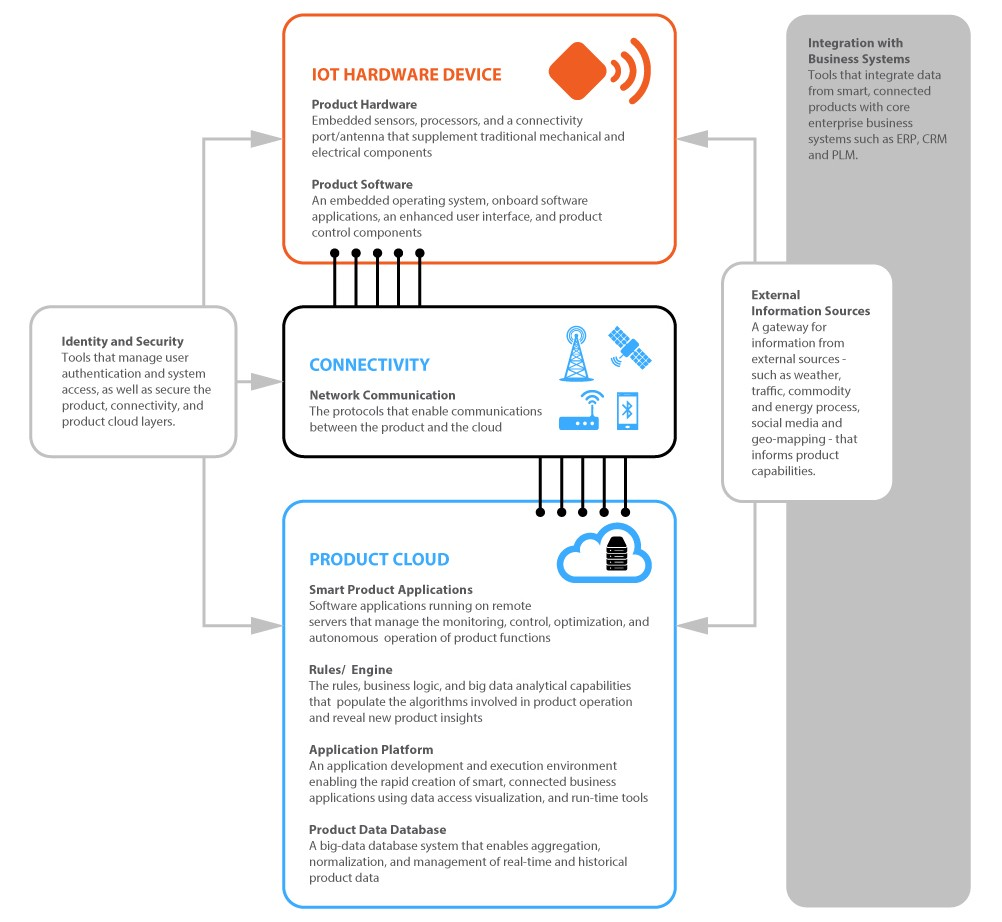
\includegraphics[trim={1cm, 0cm, 0cm, 0cm}, width=18cm, clip]{figs/iot_arch.jpeg}
\end{figure}

There are three major components of IoT project
\begin{itemize}
    \item IoT Hardware Device: the physical device that interacts with the environment
    \item Connectivity: the link between your device and the cloud
    \item {Product Cloud: servers which take data, process it, store in databases, give commands, performs analytics, serves data in a useful manner to all the different players You might be familiar with connectivity and cloud as it is the same as any website and apps. But here you will also be managing the hardware of the device which brings additional complexities.}
\end{itemize}

%%chapter IoT Hardware Device

\section{IoT Hardware Device}

This is the most complex and unique part of an IoT product. You would want to create a device-specific for you need.

For a smart irrigation system you will have to add sensors that sense moisture level and interact with pump, but for a home security system you need sensors to detect movement or cameras and process that for intruders and then alert with alarm or notifications.

One needs to select or custom-built hardware components to serve a specific use case and software that will run on this hardware.

\section{Product Hardware}

Hardware will have a central processor/controller which is responsible for logic execution and sensors and actuators which will collect data and act on commands.

Consider this central processor/controller as the brain which is responsible for all the logic and skin, eyes, hands, legs as sensors and actuators which senses and reports to brain and brain gives the command to then perform some action on the basis of that.

Based on this central unit there are microcontroller-based IoT boards and microprocessor-based boards.

\section{Microcontrollers based:}

\begin{itemize}
    \item Arduino Uno, Mega: easy to develop and lots of pins to connect peripherals, great for prototyping
    \item ESP8266 / ESP32 boards: has WiFi and Bluetooth connectivity, low cost (ESP8266 costs around \$3), plenty of resources to develop.
    \item  STM32F series boards: complex to develop, production-friendly and easily manufactured, most widely used in production.
\end{itemize}

\section{Microprocessor-based:}

\begin{itemize}
    \item Raspberry Pi: great community, easy to develop, can run OS like Linux, windows
    \item Beagle bone: open source board, can put android, ubuntu and other Linux, has built-in flash storage
\end{itemize}

\begin{figure}[!ht]
    \centering
    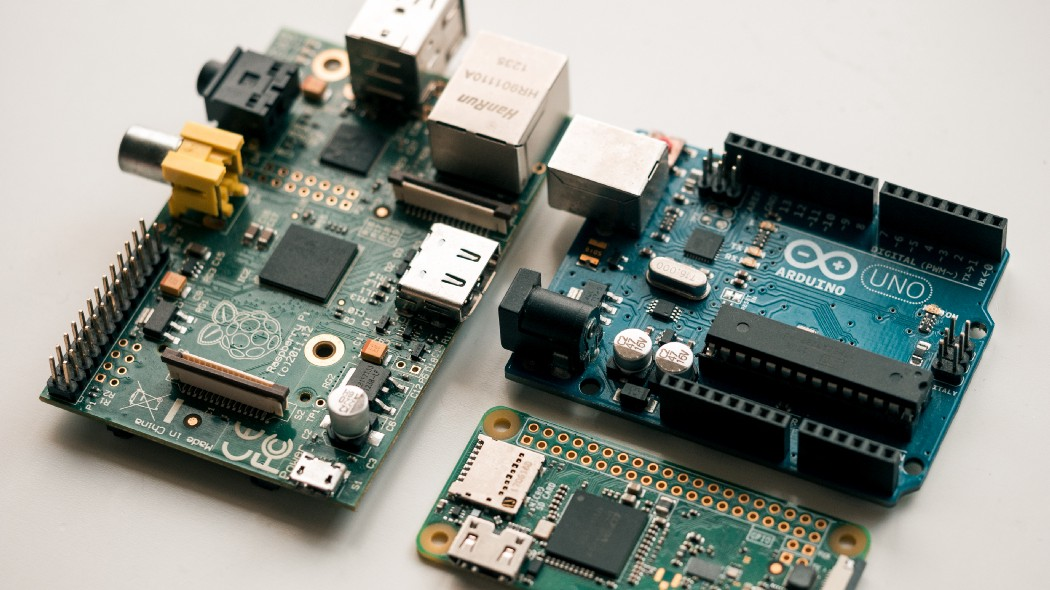
\includegraphics[trim={1cm, 0cm, 0cm, 0cm}, width=\textwidth, clip]{figs/hardware_devices.jpg}
    \caption{raspberry pi model b, raspberry pi zero, and Arduino Uno}
\end{figure}

On these boards you will notice a microcontroller and microprocessors(the big black chip in the middle). Also, there are lots of pins marked with numbers. These pins are IO pins which are used to connect to any sensors or actuators you want to use. Also if you need to use multiple microcontroller/microprocessors that can also be done as you can set up communication between those.

So just pick a board that suits your requirements and using these IO pins you can use any sensors as you like. Any sensor you pick would most probably be compatible with all the boards.

Some examples of sensors and actuators are :

\begin{itemize}
    \item Temperature and Humidity sensors
    \item Pressure Sensor
    \item Proximity Sensor
    \item Gas Sensor
    \item Smoke Sensor
    \item Alcohol Sensor
    \item Ultrasonic Sensor
    \item Relays: closing and opening the circuits electronically (switches) motors
\end{itemize}

So let’s say you want to build a fire response system, you can pick any IoT board (Arduino, ESP8266), connect smoke sensors and relay switch for the sprinkler. Whenever the smoke sensor detects smoke, give relay command to start sprinkler.
Of course you need to write this logic somewhere. That’s where product software comes in picture.

%% chapter Product Software
\chapter{Product Software and Communication Protocols}
Since the code needs to be compiled specifically for the microcontroller or microprocessor 
and due to lack of OS like Linux, Windows which abstracts the hardware variations, 
the software and tools that will be used to develop greatly depends on the chip you 
select. Though there are multiple frameworks that try to support a lot of chips.

Things you need to check out:

\begin{itemize}
    \item {Arduino Framework: supports a variety of boards and chips like all the Arduino, ESP8266, ESP32, STM32 chips}
    \item FreeRTOS: very popular OS for microcontrollers, lightweight, supports a variety of chips
    \item Amazon FreeRTOS: Amazon’s version of free RTOS which seamlessly connects to AWS IoT cloud and supports lots of other features like Over the air updates, provisioning
    \item Apache Mynewt: focused on the development of wireless-based IoT products
\end{itemize}

Also the manufacturer of the chip you select might also have some tools for development like STM offers it’s own development tools as well to develop on its chips. Be sure to check that out as well.

If you are using a more powerful IoT board like raspberry pi which can run full-fledged operating systems like Linux, Windows then of course it boils down to developing a Linux or Windows application. Though you still would need to do some hardware interactions to get data from sensors.

%% Connectivity

The choice of technology for connectivity depends on the environment you will be putting the product in. For example most home IoT will be using WiFi as it is readily available in every house, but what if you are building an air quality meter across the city wifi might not be available there you might decide to use GSM/GPRS.

Now for farming you have hundreds of sensors spread over acres you would want to use some radio communication to a central control center and then transmit all that data to the internet if needed.
So communication technologies are chosen based on use cases. Some communication technologies are :

\begin{itemize}
    \item WiFi: suitable for indoor facilities like home and office IoT devices
    \item RFID/NFC: most common use case is card-based access control
    \item GSM/GPRS: for outdoors standalone devices
    \item Bluetooth: most common choice for wearables and devices which can be controlled using a smartphone, also used for wifi provisioning ( configuring wifi credentials to a device), can also create Bluetooth mesh for multiple devices.
    \item LoRaWAN: ideal for industrial and public infrastructure products for 3–5 km range communication, designed for IoT devices, can create a network with gateways over a large area
    \item NB-IoT: Narrow Band IoT is a cellular communication technology specially designed to power IoT communication, very low power.
\end{itemize}

The next thing that comes is \textbf{Communication Protocols} that will be used for communication between your device and cloud.

\section{Messaging Communication Protocols}

\begin{itemize}
    \item HTTP: most easy to pick up, has lots of overhead, not synchronous, ideal for single requests, not continuous communication
    \item HTTP WebSockets: based on HTTP thus lots of overhead, but supports continuous communication
    \item MQTT: most commonly used IoT protocol (most solutions like Amazon FreeRTOS used this by default), based on publish/subscribe model, very lightweight, no unnecessary footprint, very flexible
    \item AMQP: open-source, message orientation, queuing, routing, supports point to point and publish-subscribe model
\end{itemize}

%% chapter Product Cloud
\chapter{Product Cloud}

Cloud is where all the processing, analysis, databases reside. When cloud receives the raw data from thousands of devices it needs to transform the data, apply business logic, store data in a manner that is useful to retrieve, and power the applications for the IoT product. It also should maintain the status, health of all the field devices. Pushover the air updates for any changes needed and keep track of which devices are updated and which are left.

Cloud is also responsible for interaction between applications (apps and websites) and the device. If any tasks or commands are given by the application, the cloud is responsible to send those commands/tasks to the devices and also should keep track whether the command is executed successfully.


To design cloud architecture these should be considered

\begin{itemize}
    \item Separate the message receiving layer from the processing layer to avoid any throttling of messages
    \item Always consider for devices going offline and malfunctioning
    \item Have provision for over the air updates (there will always be bugs and change in requirements)
    \item All communications should be secure
    \item Setup an authentication system so that once device can’t publish messages for another device and can’t subscribe to channels which are not allowed to it
    \item Keep the current state of each device in the cloud
    \item Since the size of data will get huge really soon, select a database which scales well
\end{itemize}

There are many cloud solutions which one can use :

\begin{itemize}
    \item Microsoft Azure IoT Suite
    \item Google Cloud’s IoT Platform
    \item AWS IoT Platform: integrated well with Amazon FreeRTOS
    \item Watson IoT Platform
\end{itemize}

Using a cloud would be very beneficial as it will prevent lots of designing mistakes and are built with keeping best practices in mind.

You will be bombarded with choices from device hardware, sensors, software, and communication. You have the option to choose exactly what you want and only what you need. It might be overwhelming at first, but it is really fun.

\chapter{Security of smart network}

\section{What are Some of the Risks to an Organization?}

Current IoT devices have a low degree of IT security control and weak encryption 
capabilities, leaving devices vulnerable to potential threats. 
Threat actors can take advantage of device vulnerabilities, such as in the 
following examples:

\begin{itemize}
    \item Compromising environmental control systems and smart appliances (e.g.
          coffee maker, building heating and electrical) in physical workspaces could lead to profit losses (e.g. tampering with temperature controls in a server room, causing equipment malfunction)
    \item Gaining unauthorized access to company building security controls (e.g. unlocking doors, viewing surveillance cameras)
    \item Taking control of MFDs to maliciously disrupt Internet access (e.g. Mirai botnet attack
    \item Accessing microphones remotely on IoT devices to listen in on sensitive conversations
    \item Taking control of a car’s features (e.g. tampering with a vehicle’s brakes)
    \item Controlling a hospital’s medical equipment (e.g. interfering with
          magnetic resonance imaging [MRI] systems)
    \item Accessing sensitive data or personal information (e.g. customer names
          and credit cards) through unsecured IoT devices that are connected to company networks
\end{itemize}

\section{How can I Keep IoT Devices Secure?}

Before introducing IoT devices into your organization, you should 
research security protocols and understand the types of data that the 
devices send and receive. As more IoT products are brought into the workplace, 
your organization needs plans and policies to minimize the possibility of 
cyber security incidents on your network. Your plans and policies should address 
the following considerations:

\begin{itemize}
    \item Restricting personal IoT devices to connect to a separate network (e.g. guest Wi-Fi
    \item Changing the default passwords on IoT devices. If password rules allow, use passphrases, rather than passwords, on all IoT devices in the workplace
    \item Using two-factor authentication for devices or apps to add an extra layer of security
    \item Ensuring data generated by IoT items is encrypted
    \item Turning off any automatic connection functionality (e.g. plug and play)
    \item Applying security patches and updates to IoT devices (if the product allows)
    \item Monitoring, detecting, and correcting any IoT security issues
    \item Researching reviews and security ratings on manufacturers and products
\end{itemize}

\section{IoT Best Security Practices}

\textit{One of the biggest challenges with the Internet of Things (IoT) is the security
    headache that comes with it. This issue is exacerbated in the enterprise, where 
    connected devices often control large, dangerous machines, or send and receive 
    sensitive data. While the IoT can bring new data and helpful insights, it also 
    introduces new vulnerabilities into your organization. As such, it’s critical 
    that enterprises consider the security implications of an IoT deployment before 
    moving forward.}

Securing an IoT infrastructure requires a rigorous security-in-depth strategy. 
This strategy requires you to secure data in the cloud, protect data integrity 
while in transit over the public internet, and securely provision devices. 
Each layer builds greater security assurance in the overall infrastructure.
According to the IEEE document on IoT security the best practices for businesses, 
schools, factories, and other organizations looking to improve their IoT security are:

\section{Making hardware tamper-resistant}

Some IoT devices may operate continuously unattended and not subject to the security 
implied by this frequent, direct human observation. While it is best to keep devices 
relatively isolated so that only a few designated persons have physical access, 
especially for completely unattended devices, making them tamper-proof or 
tamper-evident may be advantageous. This form of endpoint hardening can help 
block potential intruders from reaching data. It may also defend against a hacker 
buying and then weaponizing devices. The physical security of endpoints can include, 
for example, small simple plastic devices, port locks, and camera covers, 
which lockout USB and Ethernet ports and cover webcam apertures. 
Port locks help prevent unwanted malware from coming in. Some tamper-resistive 
approaches disable the device when it is tampered with. As a best practice, 
secure endpoint hardening likely implies a layered approach that requires 
attackers to circumvent a variety of obstacles designed to protect the device 
and its data from illicit access and use. At the hardware/boot-software level, 
strong boot-level passwords or requiring the device to boot from local storage 
only maybe sound approaches. Known vulnerabilities should be protected, such as 
open TCP/UDP ports, open serial ports, open password prompts, places to inject 
code such as web servers, unencrypted communications and radio connections. 
For shipping, tamper-evident packaging will enable the device owner to know if a 
device has been opened before it arrived. The number and strength of security at 
each layer depend upon the threat model, acceptable levels of risk, and desired 
convenience.

\section{Provide for firmware updates/patches}

Inevitably vulnerabilities will be discovered after devices have been deployed. 
Devices must be patchable or upgradable. Naturally, device firmware should only 
be modifiable with the proper digital signature. As it stands, device vendors and 
manufacturers have a little financial incentive in ensuring ongoing IoT patch 
upgrades since revenue comes from the sale of the device, not the maintenance. 
The upkeep of IoT devices may detract from revenue. In addition, vendors are not 
legally held accountable for ongoing maintenance of devices beyond initial sales 
and competition drives vendors to cut corners, negating on quality for efficiency 
and speed of release into the market. While these factors may not have been critical 
previous to IoT, the interconnected nature of IoT devices raises the bar to a new 
level in terms of functionality and accountability. Detrimental also is the 
tendency of vendors towards planned obsolescence of devices in order to maximize 
profit through continued sales rather than through the upkeep of existing devices. 
Furthermore, IoT devices are not efficiently designed or configured to respond to 
OTA (over the air) updates, resulting in, at best costly, and at worst, unmanageable 
procedures. As it stands, many IoT devices are un-patchable, and as such, cannot 
be made secure. Researchers have observed that the ubiquitous advancement of IoT 
and the placement of unsecured and unattended IoT devices throughout homes and 
businesses will increase exponentially, opening up opportunities for hackers 
to exploit critical vulnerabilities [9]. Further to planned obsolescence, many 
IoT devices simply have limited life cycles. Companies must be legally held 
accountable to monitor and maintain devices through prescribed and agreed 
upon lifecycles. For this, there needs to be standards established and 
legislation put in place. In addition, vendors need to remain transparent 
and forthcoming about the life cycle of devices, especially in terms of service 
and upkeep policies, including the length of time they plan to support their devices. 
They need to take an active role in providing details on patches and upgrades as well 
as security risks and privacy concerns, ensuring that the consumer and/or user is 
informed about changes in policy, functionality, and security. 
The full lifecycle of the IoT device must be considered, beginning at manufacturing 
where security credentials must be “generated, allocated, and provisioned into 
the devices in a secure manner” [8]. Deliberations must also integrate the 
lifecycle of the original manufacturer. When the original vendor no longer exists, 
it becomes impossible to trace credentials in order to patch vulnerabilities and 
security breaches, and vendors are inevitably replaced and/or go defunct or bankrupt.

\section{Perform dynamic testing}

It is crucial that IoT devices undergo thorough testing, and establish a 
minimum baseline for security. Static testing is not intended or designed 
to find vulnerabilities that exist in the off-the-shelf components such as 
processors and memory into which may be a component of the overall application. 
Dynamic testing, on the other hand, is capable of exposing both code weaknesses 
and any underlying defects or vulnerabilities introduced by hardware and which may 
not be visible to static analysis. Dynamic testing may discover vulnerabilities that 
are created when a new code is used on old processors. We recommend manufacturers 
who purchase hardware and software from others do dynamic testing to ensure the 
items are secure.

\section{Specify procedures to protect data on device disposal}

Eventually, devices become obsolete and users may decide to throw them away. 
Devices should be discarded without exposing private data. This is a security 
issue because improperly discarded devices may be converted to serve malicious 
purposes. This is a privacy issue because, if left in operation or if disposed of 
improperly, obsolete hardware could be used to reveal personal information about 
the user or other stakeholders in the IoT ecosystem. The same will be true for 
IoT devices that are sold to second owners or that become standard equipment in 
homes and are conveyed upon the sale of the house. We suggest manufacturers prepare 
a formal plan for users to sanitize and dispose of obsolete IoT devices. Industry 
practice in other fields prescribes a “discard, recycle or destroy” (DRD) policy 
with periodic review of the plan to determine which devices require disposal and 
how to dispose of them. Some manufacturers encourage users to dispose of products 
directly through the manufacturer. This may be sensible for laptops and servers, 
but for IoT devices that may be small and cheap, or that are part of a much larger 
device (like a refrigerator) special accommodations may be required. Individual 
users, when purchasing a used IoT product, might attempt to identify what personally 
identifiable information (PII) or authentication information such as username and 
password (UNPW) remains stored on the device, or is accessible by the device, or 
is required to be stored elsewhere in order to use the device. For example, 
the Amazon Echo Dot requires users to store their Wi-Fi network router passwords 
on an Amazon server. The question must be asked whether users should be expected 
to determine an individual DRD policy or not, which may include deleting information 
from any Internet-accessible location other than the device itself. As it stands, 
users are inadequately prepared, not possessing the digital skills needed to navigate 
this kind of level of security, and being ill-equipped to understand the complexities 
of password storage in connected devices. Exposure of such complexities often comes 
too late, as was the case in the recent revelation that modern copiers and fax 
machines have hard drives that retain copies of documents. Even corporate users 
with IT departments trained in security were unaware of this fact. 
The implications for security in the above example are numerous and highlight 
how easy it is for major security flaws to be left unaccounted for.

\section{Use strong authentication}

IoT devices should not use easy-to-guess username/password credentials, such as 
admin/admin. Devices should not use default credentials that are invariant across 
multiple devices and should not include back doors and debug-mode settings 
(secret credentials established by the device’s programmer) because once guessed, 
they can be used to hack many devices. Each device should have a unique default 
username/password, perhaps printed on its casing, and preferably resettable by the 
user. Passwords should be sophisticated enough to resist educated guessing and 
so-called brute force methods. Where possible we recommend two-factor authentication 
(2FA), which requires a user to employ both a password and another authentication 
form that does not rely on user knowledge, such as a random code generated via SMS
text messaging. For IoT applications, we especially encourage the use of 
context-aware authentication (CAA), also known as adaptive authentication, 
in which use contextual information and machine-learning algorithms continuously 
evaluate the risk of malice without bothering the user in demanding authentication. 
If the risk is high, then the subscriber (or hacker) would be asked for a 
multi-factor token to continue having access.

\section{Use strong encryption and secure protocols}

Even if device passwords are secure, communications between devices may be hackable. 
In the IoT, there are many protocols, including Bluetooth, Zigbee, Z-Wave, 6LoWPAN, 
Thread, Wi-Fi, cellular, NFC, Sigfox, Neul, and LoRaWAN. Depending on the protocol 
and on available computing resources, a device may be more or less able to use strong 
encryption. Manufacturers should examine their situation on a case-by-case basis and 
use the strongest encryption possible, preferably IPsec and/or TLS/SSL. There may be 
cases where encryption is not desirable, such as in SAE J2735 Basic Safety Messages 
(BSMs), the wireless communications cars can use to avoid collisions. In those cases, 
messages can be sent in the open and verified using digital signatures. However, 
consideration should be given to the implications of omitting encryption. In the 
SAE J2735 case, BSMs could be used to alert collision-management systems falsely 
and immobilize an automobile. There is no stock answer that avoids the need for 
careful thought about the threat models anticipated and the vulnerabilities that 
will be tolerated. If data are transmitted unencrypted and unsigned, precautions 
should be made to ensure that false data have little or no chance of causing harm.

\section{Minimize device bandwidth}

Recently DDoS attacks have been conducted in large measures by armies of poorly 
protected IoT devices that have become zombie systems in massive global campaigns. 
Most IoT devices are made of commodity components that have vastly overpowered network 
capabilities for the function they are supposed to perform causing congestion on home 
networks and potentially contributing to huge costs for the targets of IoT-borne DDoS 
attacks. If in the future there were 50 billion devices connected to the Internet, 
and if we assume (based on current conditions) that 1.1\% of them are compromised and 
under coordinated remote control, that is 55 million rogue IoT devices. 
Suppose each device is capable of generating line-rate attack traffic equivalent 
to Gigabit Ethernet (81,274–1,488,096 frames per second), for example, 
the ARM9 system-on-a-chip (SoC) has two such connections built-in, and it costs 
less than \$5 to make per chip. Using this 55-million-device zombie army to generate 
DDoS events, attackers could generate between 4.47 to 81.8 trillion frames per second 
or 55 petabits per second. This is well beyond the defensive capabilities of any 
single service provider. An attack of this magnitude would overwhelm the fastest 
network interface built to date (300Gbps) by a margin of 183,333 to 1. 
There is no good way to reduce the malicious traffic produced by these systems
apart from squelching it at the source. We recommend device manufacturers should 
limit the amount of network traffic IoT devices can generate levels reasonably 
needed to perform their functions. There is very little need for an Internet-connected 
refrigerator to spew Internet Control and Management Protocol (ICMP) messages at 
gigabit-per-second speeds. While some refrigerators are outfitted with video screens, 
they more than likely do not need to have high-speed upload capabilities. 
Vendors should use hardware and kernel-level bandwidth limitations to throttle 
network transmission rates to levels reasonable for the tasks of each device. 
Such limitations make it much harder for an attacker to use a device in a DDoS 
attack, even if he has completely compromised it. Additionally, devices should 
be programmed to self-monitor for unusual behaviors and restore themselves to 
factory settings when alarming behavior is detected. If resetting devices to factory 
settings is not feasible, devices should at least reboot to potentially clear code 
the attacker has running in memory. Now, supposing the aforementioned 55 million 
malicious IoT devices had hardware/kernel-enforced attenuated bandwidth, 
say 10 Ethernet frames per second, then their aggregate potential attack profile 
drops to 550 million frames per second, and not more than 6.6 terabits per second. 
This nearly 150,000 times smaller, and while it is still too big for a single defender,
that size attack is feasible for a distributed set of defenders to stop. 
Additional kernel-level controls within devices that notice and attenuate large 
amounts of uploaded traffic or stop other unexpected behavior could further reduce 
the destructive capabilities of compromised devices without requiring heroic 
efforts by network defenders. Thus, we recommend serious consideration of 
the performance requirements of each device and that modest limitation be 
emplaced that are difficult to circumvent. This will greatly increase the 
safety of IoT devices and make it possible to safely field many more of them in 
the future.

\section{Divide networks into segments}

Separate the network into smaller local networks using VLANs, IP address ranges, or a 
combination thereof. Network segmentations are utilized in next-generation firewall 
security policies to clearly identify one or more source and destination interfaces 
on the platform. Each interface on the firewall must be assigned to a security zone 
before it can process traffic. This allows organizations to create security zones to 
represent different segments being connected to and controlled by, the firewall. 
For example, security administrators can allocate all cardholder or patient data 
repositories in one network segment identified by a security zone (e.g., Customer Data).
Then the administrator can craft security policies that only permit certain users, 
groups of users, specific applications, or other security zones to access the 
Customer Data zone — thereby preventing unauthorized internal or external access 
to the data stored in that segment. This type of solution is more common in industrial 
applications but may be useful in broader circumstances. A separate, detached private 
network for a security system, perhaps with a dedicated channel to a “home base” in 
the case of a home security system, might suffice. If the system must use the Internet, 
a virtual private network (VPN) might be implemented.




\end{document}




